\chapter{Reproduktion bisheriger Ergebnisse}
\label{chap:reproduktion}
\epigraph{What I cannot create, I do not understand}{--- Richard Feyman}

\qq{welche Experimente?}
Ziel 
Im folgenden werden Paper genauer untersucht, die sich mit dem Problem der Dokumentensegmentierung mit Hilfe von CNNs nähern.
Das erste Experiment basiert auf dem neusten Paper von Mitgliedern der DIVA-Gruppe: \citeauthor*{ChenConvolutionalNeuralNetworks2017}. 

Das zweite Experiment basiert auf der Forschung des Gewinners des IDCAR2017-Wettbewerbs: \citeauthor*{XuPageSegmentationHistorical2017} 

Beide Untersuchungen benutzen den gleichen Datensatz als Grundlage für ihre Experimente. 
\section{Andere Ansätze}
\cite{WickFullyConvolutionalNeural2017}
Im Bereich der Bibliotheswissenschaften besteht ein großes Interesse an Klassifizierung von
Buchseiten zur besseren Erschließung.
\cite{McConnaugheyLabeledSegmentationPrinted2017} klassifizieren Buchseiten anhand von textbasierten Features in 4 Kategorien. 


% Kontext/prior work
% Prozessbeschreibung
% Vorverarbeitung
% Netzarchitektur
% Training 
% Nachverarbeitung


\section{Datensatz}

\section{Auswahl und Beschreibung des Datensatzes}
\textcite[985\psqq]{DoermannHandbookdocumentimage2014} listen 5 Aspekte die bei der Erstellung von Datensätzen zu beachten sind:
\begin{itemize}
    \item Auswahl der Daten
    \item Datenbeschaffung
    \item Ground Truth Definition
    \item Ground Trouth Annotation
    \item Speicherformat
    \item Struktur und Organisation
\end{itemize}

\section{DIVA-HisDB}
Die DIVA \marginnote{\url{http://diuf.unifr.ch/main/diva/}} (Document, Image and Voice Analysis) Gruppe der Universität Fribourg hat im Kontext der Forschungsprojekte HisDoc und HisDoc 2.0 
das Datenset DIVA-HisDB. erstellt.
Die HisDoc-Projekte beschäftigen sich mit der automatischen Analyse von historischen Dokumenten und
wie man diese für Historiker nutzbar machen kann.

\cite{SimistiraDIVAHisDBPreciselyAnnotated2016}

% Auswahl der Daten
Für den Datensatz wurden Dokumente mit komplexen Layout aus der Virtuellen Manuskriptbibliothek der Schweiz (\url{http://www.e-codices.unifr.ch/en}) ausgesucht. 
\research{Manuskriptbibliothek}

% Struktur und Organisation 
Die Manuskripte enthalten neben dem Haupttext auch Randnotizen und Text-Dekorationen. 
Randnotizen befinden sich auch teilweise zwischen den Zeilen des Haupttexts.
DIVA-HisDB besteht aus 150 Dokumenten, aufgeteilt in Trainings-, Validierungs- und Testset (siehe \cref{table:hisdb_pages}. 
Hinzu kommen 30 Seiten die für die finale Wertung des Wettbewerbs ``ICDAR2017 Competition on Layout Analysis for Challenging Medieval Manuscripts'' verwendet wurden.

\begin{table}
    \caption{Aufteilung der Seiten des DIVA-HisDB-Datenssets}
    \label{table:hisdb_pages}
    \begin{tabular}{lccccc}
        {\bfseries Name} & {\bfseries Auflösung} & {\bfseries Training} & {\bfseries Validierung} & {\bfseries Test} & {\bfseries Test ICDAR 2017)}\\
        \csvreader[head to column names]{tables/diva_hisdb_specs.csv}{}%
        {\name&	\width \(\times\)\height & \train	&\validate	&\test	&\comp\\}
    \end{tabular}
\end{table}

% Datenbeschaffung
Alle Daten können direkt von der Webseite der DIVA-Gruppe heruntergeladen werden.

% Speicherformat
Die Manuskripte wurden mit einer Auflösung von 600 dpi gescannt und sind im  JPEG-Format gespeichert. 
Die \cref{table:hisdbsamples} zeigt Beispiele aus den drei Datensätzen. 

% Ground Truth Definition
Der Datensatz wurde semi-automatisch mit 3 Annotation (Haupttext, Kommentare, Dekorationen) versehen.
Alle Bereiche die nicht annotiert sind werden als Bildhintergrund betrachtet.

% Ground Trouth Annotation
Diese Ground-Truth-Annotationen sind im PAGE-XML-Format und als ``pixel-label'' PNG-Bilder gespeichert.
Die \cref{fig:ground_truth} zeigt eine Beispielseite mit den zugehörgine Labels auf Pixelebene. 

\begin{figure*}
    \centering
    \caption{Hintergrund: weiss, Haupttext: blau, Kommentare: grün, Dekorationen: rot }
    \label{fig:ground_truth}
    \subfloat[Dokumentenbild]{%
        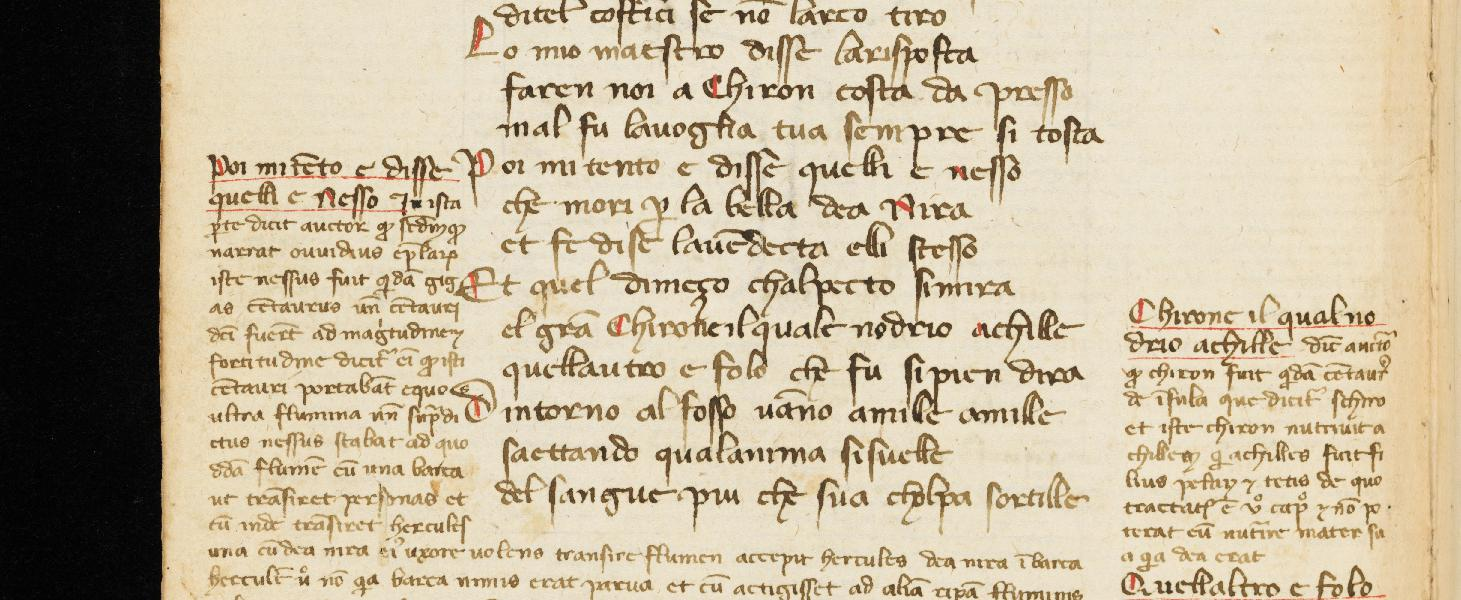
\includegraphics[width=0.5\textwidth]{figures/datasets/gt_example0.jpeg}
    }
    \subfloat[``pixel-label'']{%
        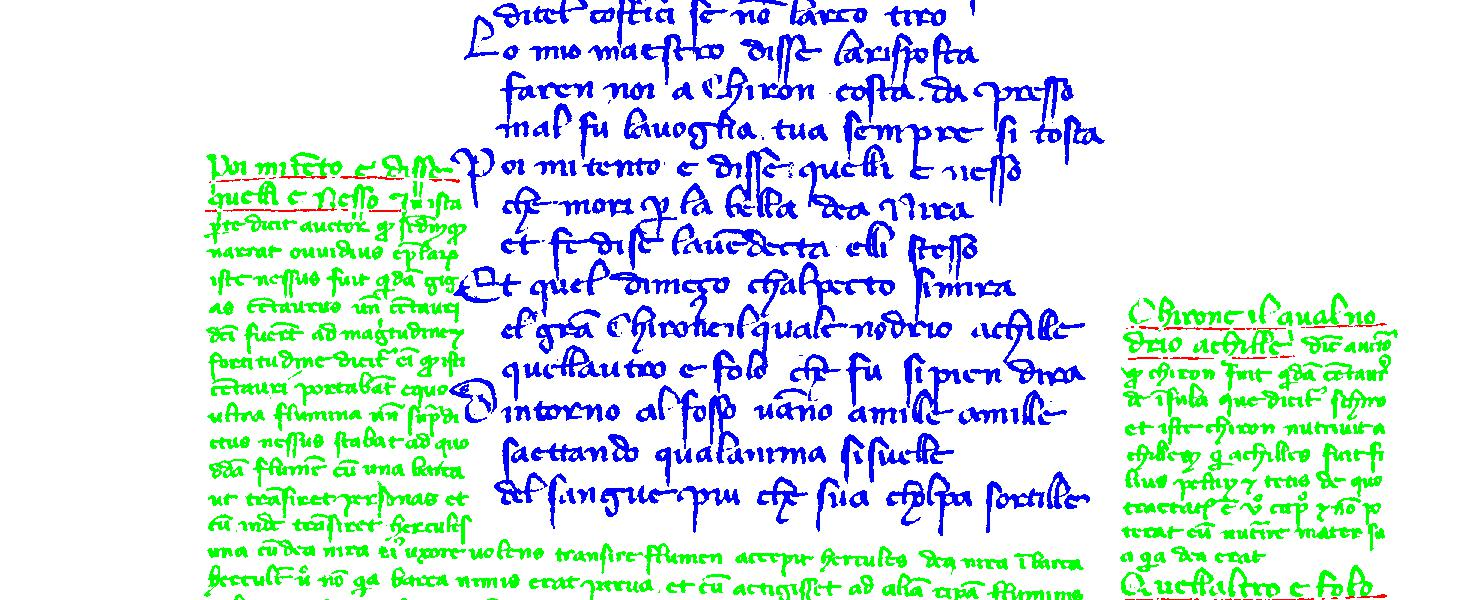
\includegraphics[width=0.5\textwidth]{figures/datasets/gt_example1.jpeg}
    }
\end{figure*}

Die Menge an Pixeln pro Klasse ist sehr unterschiedlich.
Die \cref{table:class_distribution} zeigt das in jedem Dokumentenset der Hintergrund deutlich überwiegt.

\begin{table}
    \caption{Verteilung der Klassen in Prozent\autocite[1362]{SimistiraICDAR2017CompetitionLayout2017}}
    \label{table:class_distribution}
    \begin{tabular}{lrrrr}
        {\bfseries Set} & {\bfseries Hintergrund} & {\bfseries Kommentar} & {\bfseries Dekoration} & {\bfseries Text}\\
        \csvreader[head to column names]{tables/diva_hisdb_class_distribution.csv}{}%
        {\set&	\background & \comments & \decoration & \text \\}
    \end{tabular}
\end{table}



\begin{table*}
    \begin{tabular}{llp{4cm}}
        \vspace{0.2cm}
        {\bfseries Seite} & {\bfseries Detailauschnitt} & {\bfseries Quelle } \\
        \vspace{0.5cm}
        
        \raisebox{-.5\height}{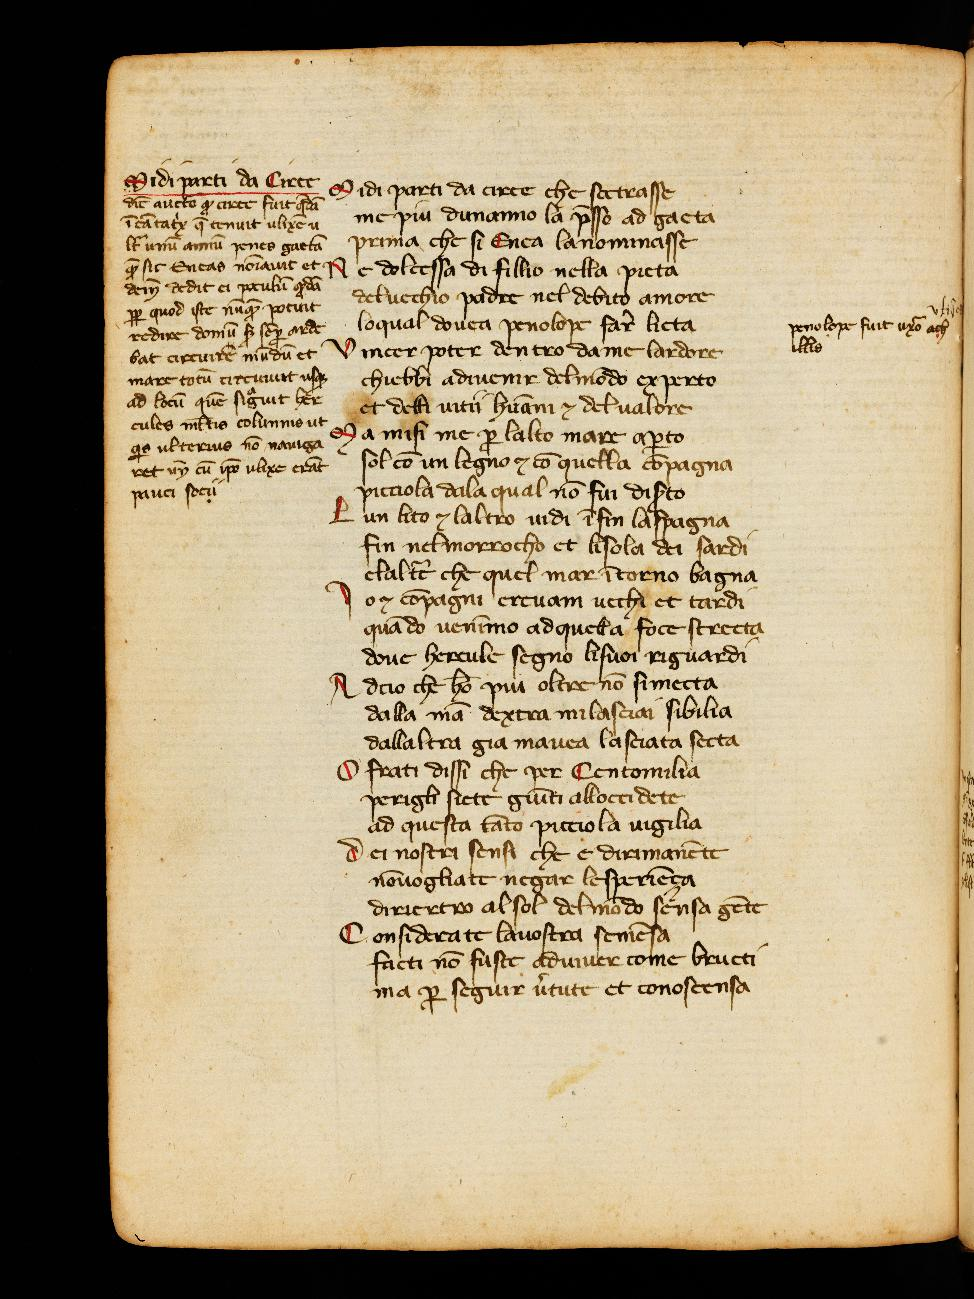
\includegraphics[height=4cm]{figures/datasets/HisDBSample0.jpeg}}
    &\raisebox{-.5\height}{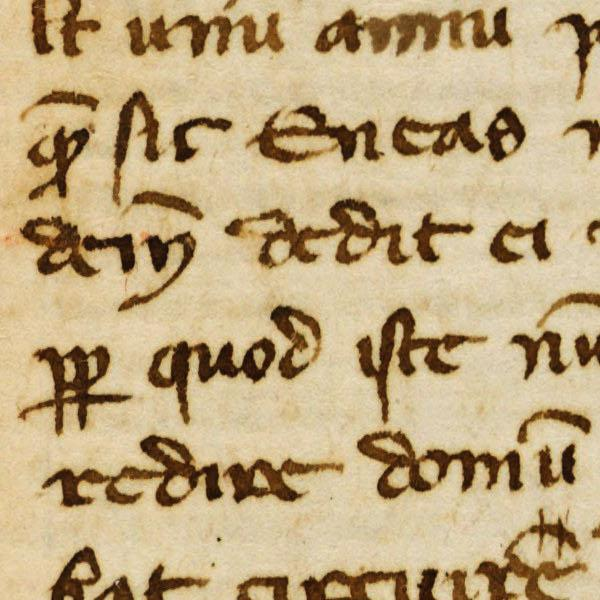
\includegraphics[height=4cm]{figures/datasets/HisDBSampleBox0.jpeg}}
     & \citefield{AlighieriColognyFondationMartin1300}{title}\\
     \vspace{0.5cm}  
     
    \raisebox{-.5\height}{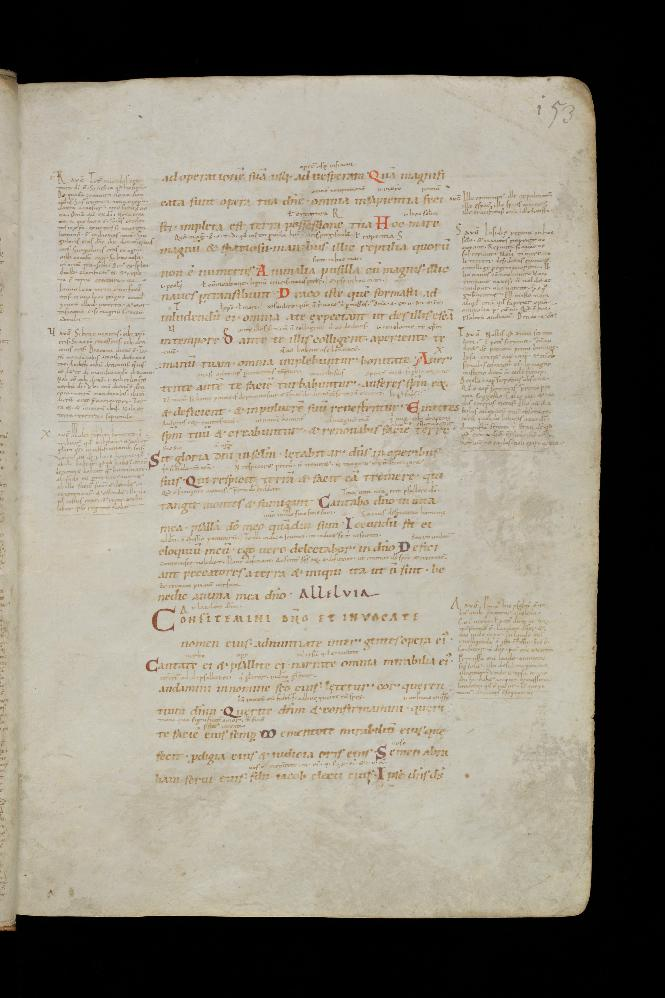
\includegraphics[height=4cm]{figures/datasets/HisDBSample2.jpeg}}
    & \raisebox{-.5\height}{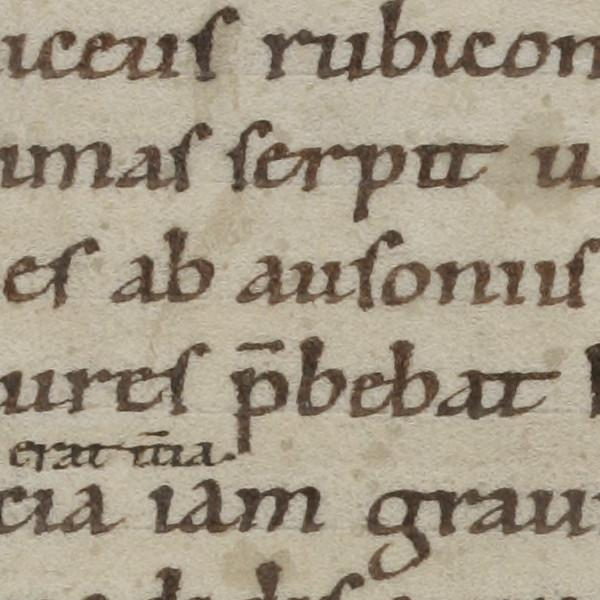
\includegraphics[height=4cm]{figures/datasets/HisDBSampleBox2.jpeg}}
    & \citefield{AmbrosiusStGallenStiftsbibliothek985}{title}\\
    \vspace{0.5cm}
    
     \raisebox{-.5\height}{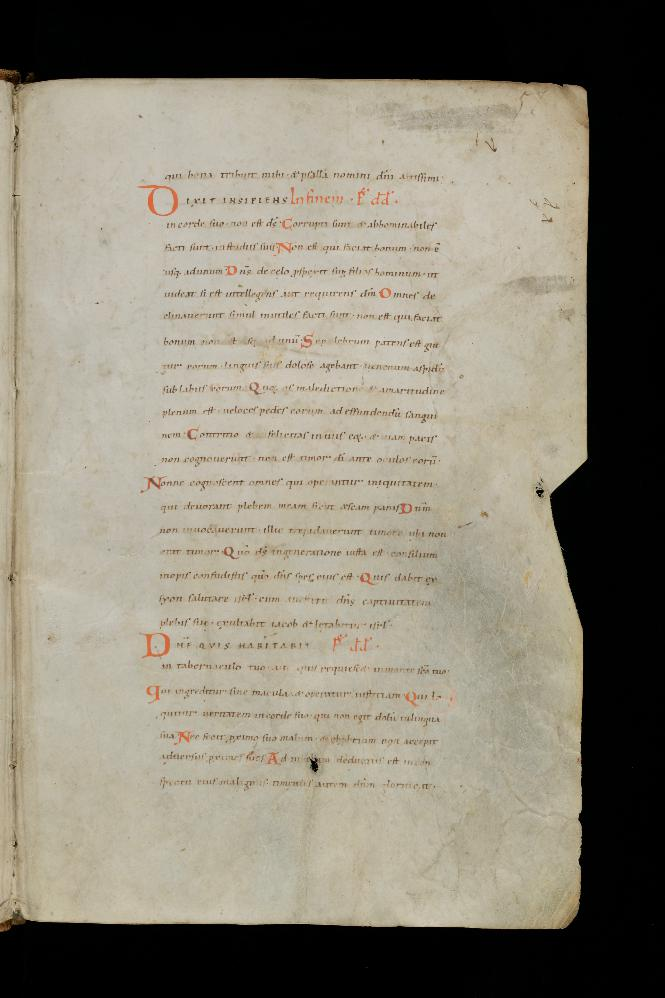
\includegraphics[height=4cm]{figures/datasets/HisDBSample1.jpeg}}
    &\raisebox{-.5\height}{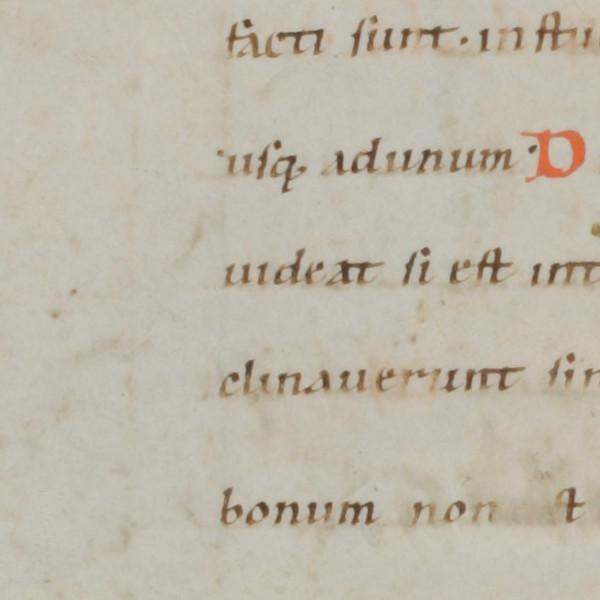
\includegraphics[height=4cm]{figures/datasets/HisDBSampleBox1.jpeg}}
     & \citefield{LucanusStGallenStiftsbibliothek1025}{title}\\
     \vspace{0.5cm} 

    \end{tabular}
    \caption{HisDB Beipsiele mit Detailauschnitt}
    \label{table:hisdbsamples}
\end{table*}

\subimport{reproduktion/}{chen}
\section{\textcite{XuPageSegmentationHistorical2017}}
Das Paper \citetitle*{XuPageSegmentationHistorical2017} von \citeauthor*{XuPageSegmentationHistorical2017} verfolgt einen anderen Ansatz.
\citeauthor{XuPageSegmentationHistorical2017} verwenden eine Netwerk  


\section{VGG}


\section{Deconvolution}

\section{Ergebnisse}